\section{Design}
\label{sec:design}

The design of the Capri-based \atl can be separated into four parts: knob
selection, feature selection, the offline training phase and the online testing
phase. Knobs, as descried
The offline training phase captures
the characteristics of the platform features and knob settings by doing
exhaustive runs. Capri uses the profiling data and builds a model for the \gem
performance based on featues and knobs. In the testing phase, the model takes
a platform and a ``top M'' constraint as input, and output the best predicted
knob setting for GEMM for this platform.

  \subsection{Knob selection}
  \label{sec:knobs}

  \subsection{Feature selection}
  \label{sec:features}
  Features are used in Capri as the identification for different inputs.

  \subsection{Offline Training}
  \label{sec:offline_training}

  \subsection{Online Testing}
  \label{sec:online_training}

\begin{figure*}[tbhp]
  \centering
  \begin{subfigure}[b]{1.0\linewidth}
    \centering
    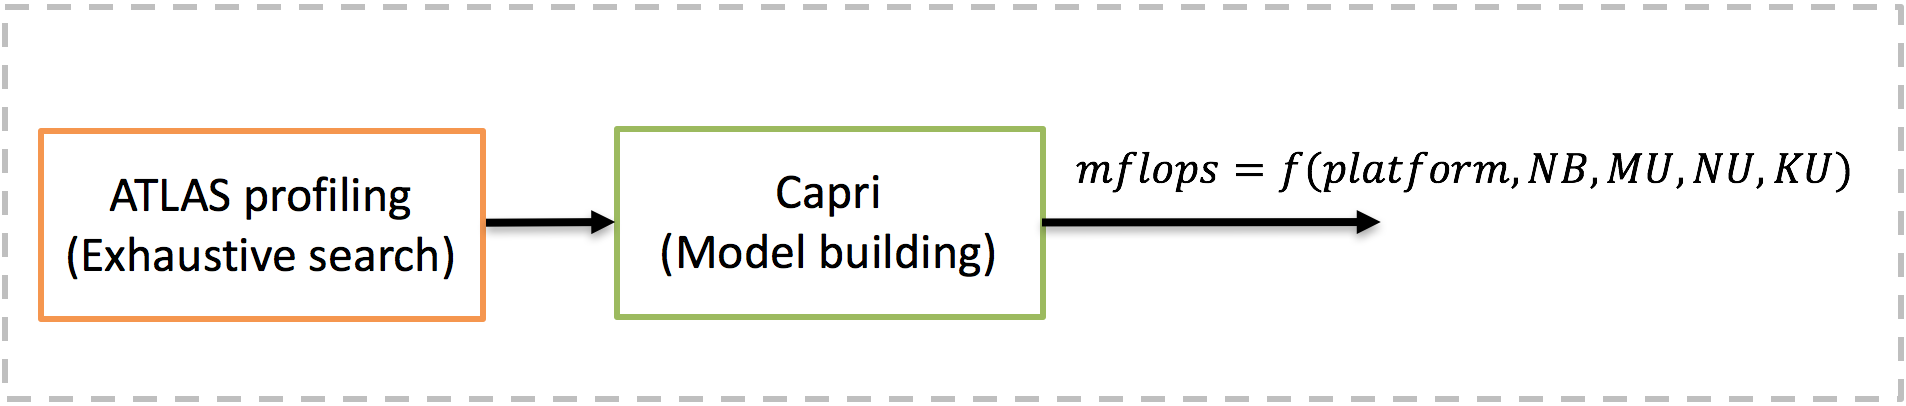
\includegraphics[width=0.9\textwidth]{images/offline_training.png}
    \caption{Offline training phase: \atl profiling and Capri model building}
  \end{subfigure}
  \begin{subfigure}[b]{1.0\linewidth}
    \centering
    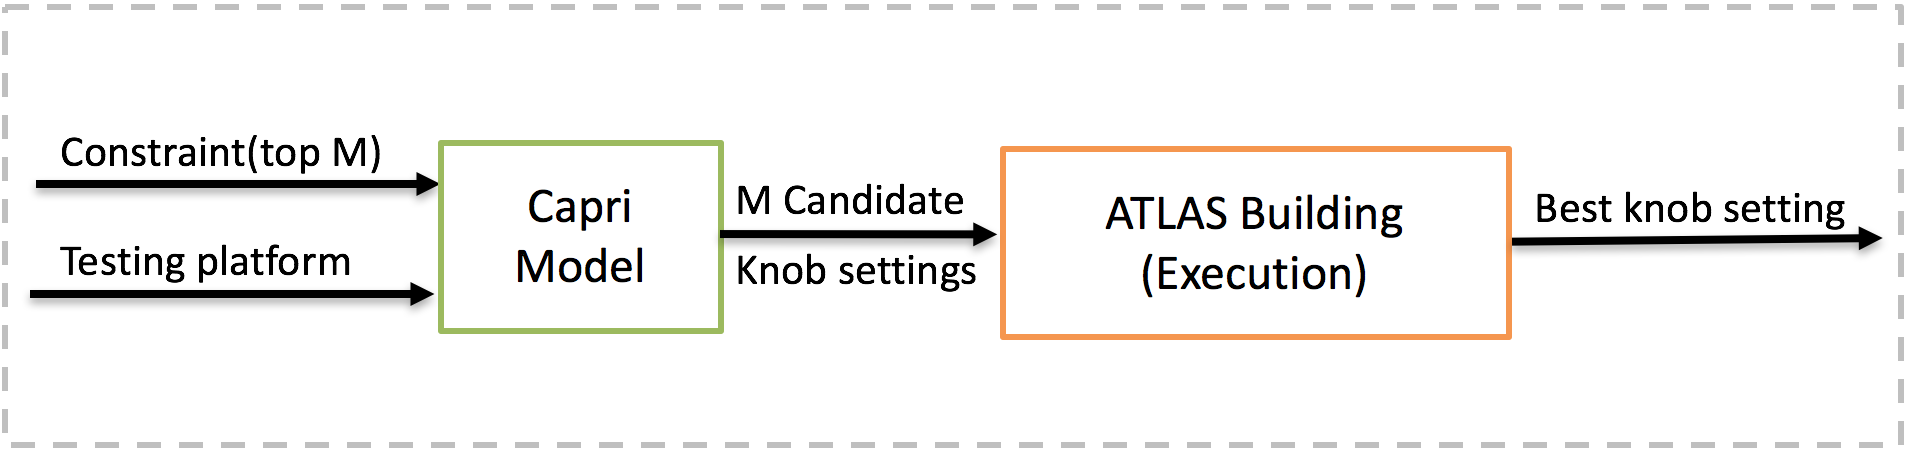
\includegraphics[width=0.9\textwidth]{images/testing.png}
    \caption{Online testing phase: Capri model searching and \atl execution}
  \end{subfigure}
  \caption{Capri-based \atl design diagram}
  \label{fig:design}
\end{figure*}

$mflops = f(platform, NB, MU, NU, KU)$
